\documentclass[dvipdfmx]{jarticle}%% 図の表示にdvipdfmxの指定が必要
\usepackage[dvipdfmx]{pict2e}
\usepackage{ketpic2e}
\usepackage{ketlayer2e}
\usepackage{amsmath,amssymb}
\usepackage{graphicx}%% ここでdvipdfmxを指定してもダメ,documentclasseで指定
\usepackage{xcolor}

\setmargin{20}{20}{20}{20}

\begin{document}
背景色を変えるには。\\

\begin{layer}{170}{0}
\putnotesw{80}{00}{図1}%%図のファイル名に全角文字を含めない
\putnotesw{130}{00}{図2}
\putnotesw{80}{40}{図3}
\putnotesw{130}{40}{図4}
\putnotesw{120}{00}{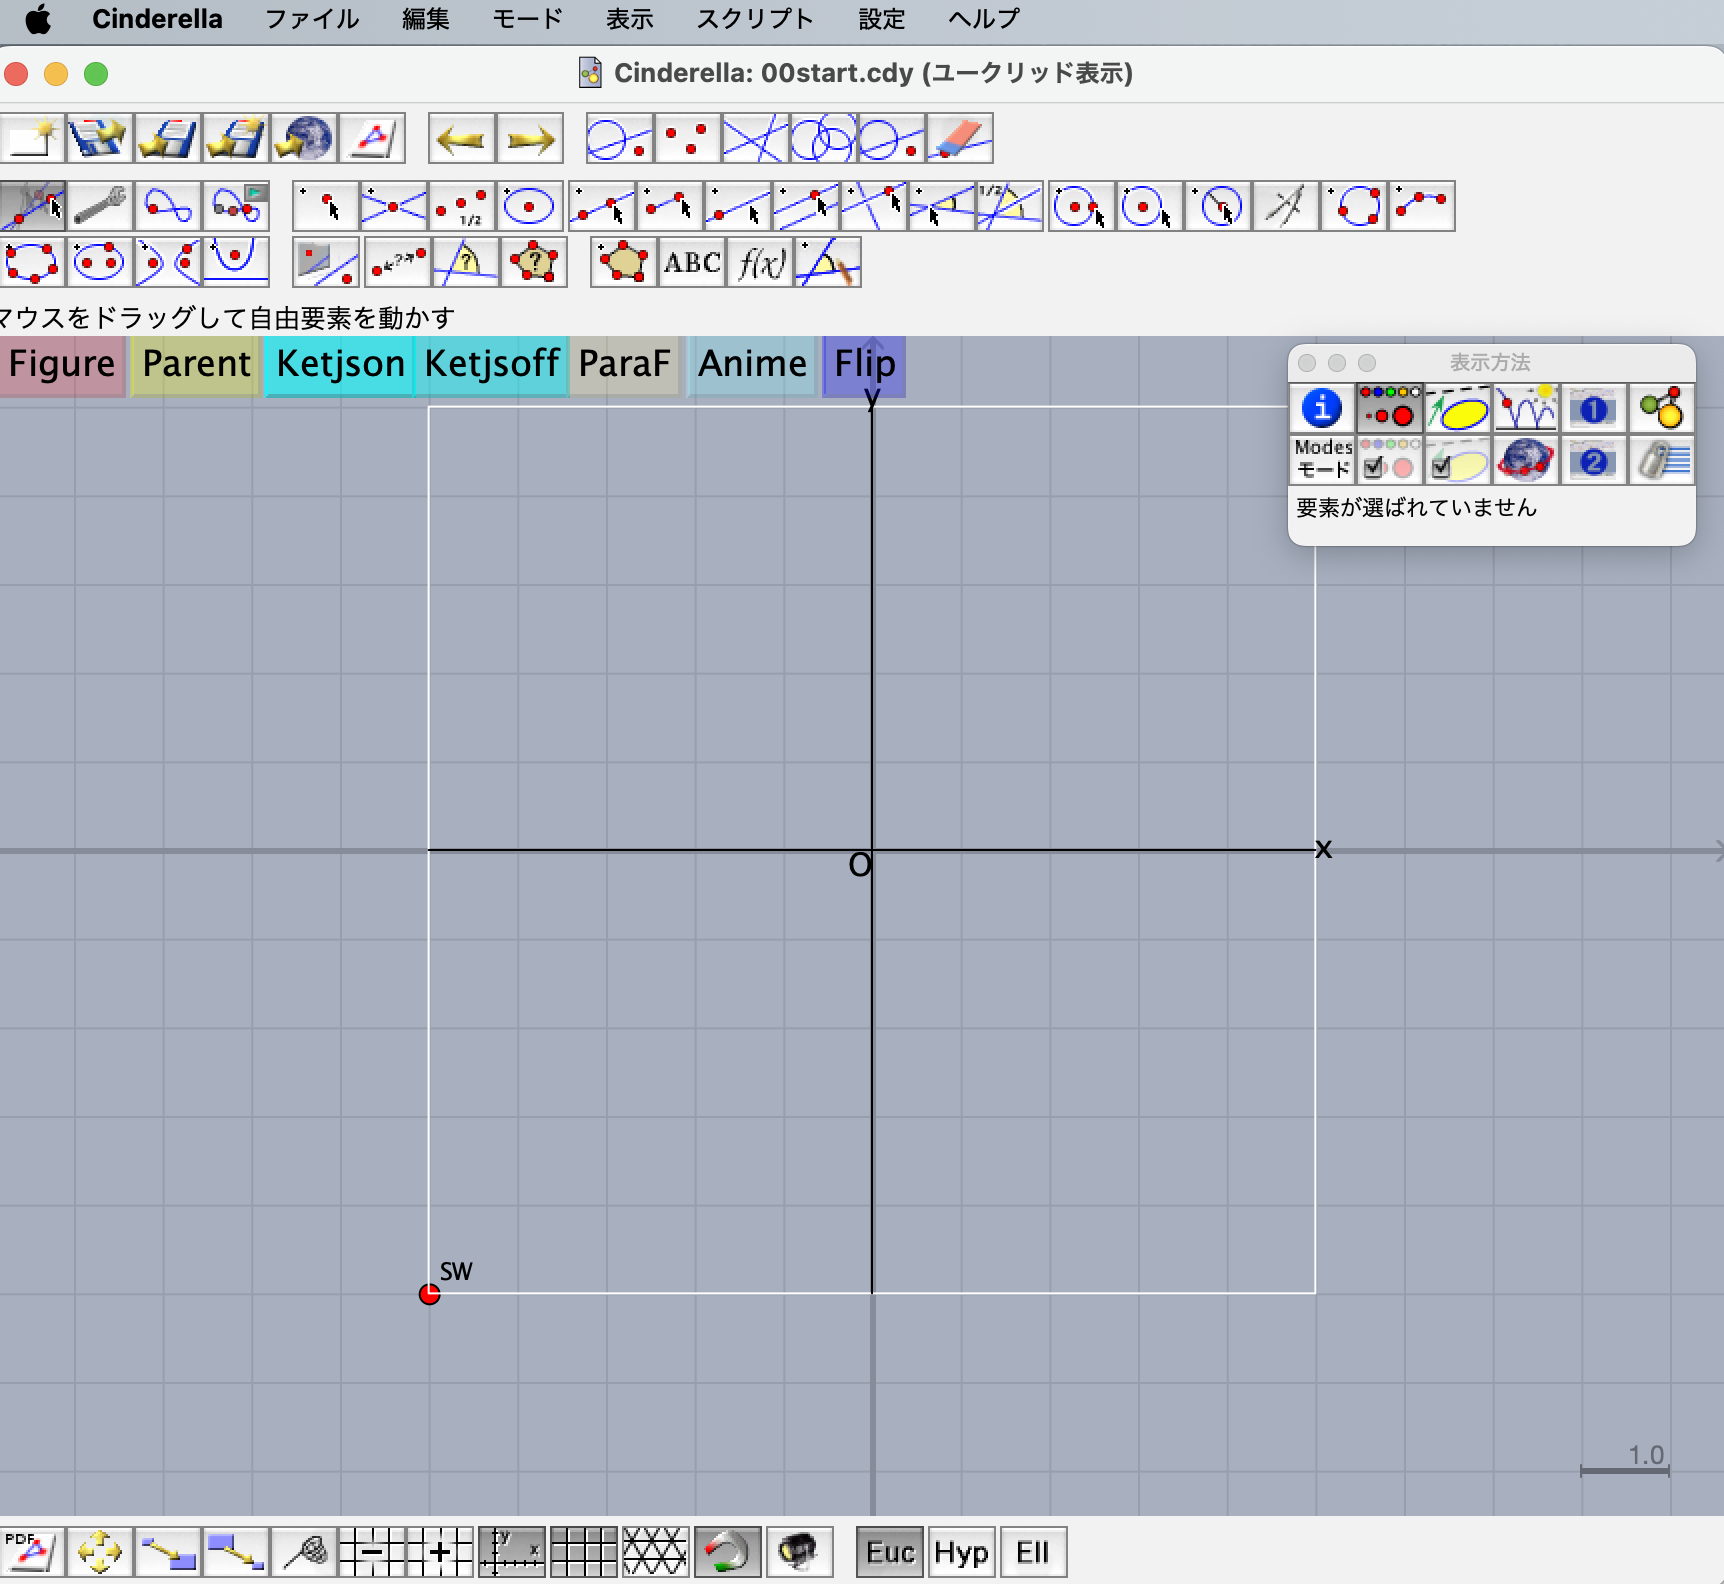
\includegraphics[bb=0 0 1724 1584,width=38mm]{1.png}}
\putnotesw{170}{00}{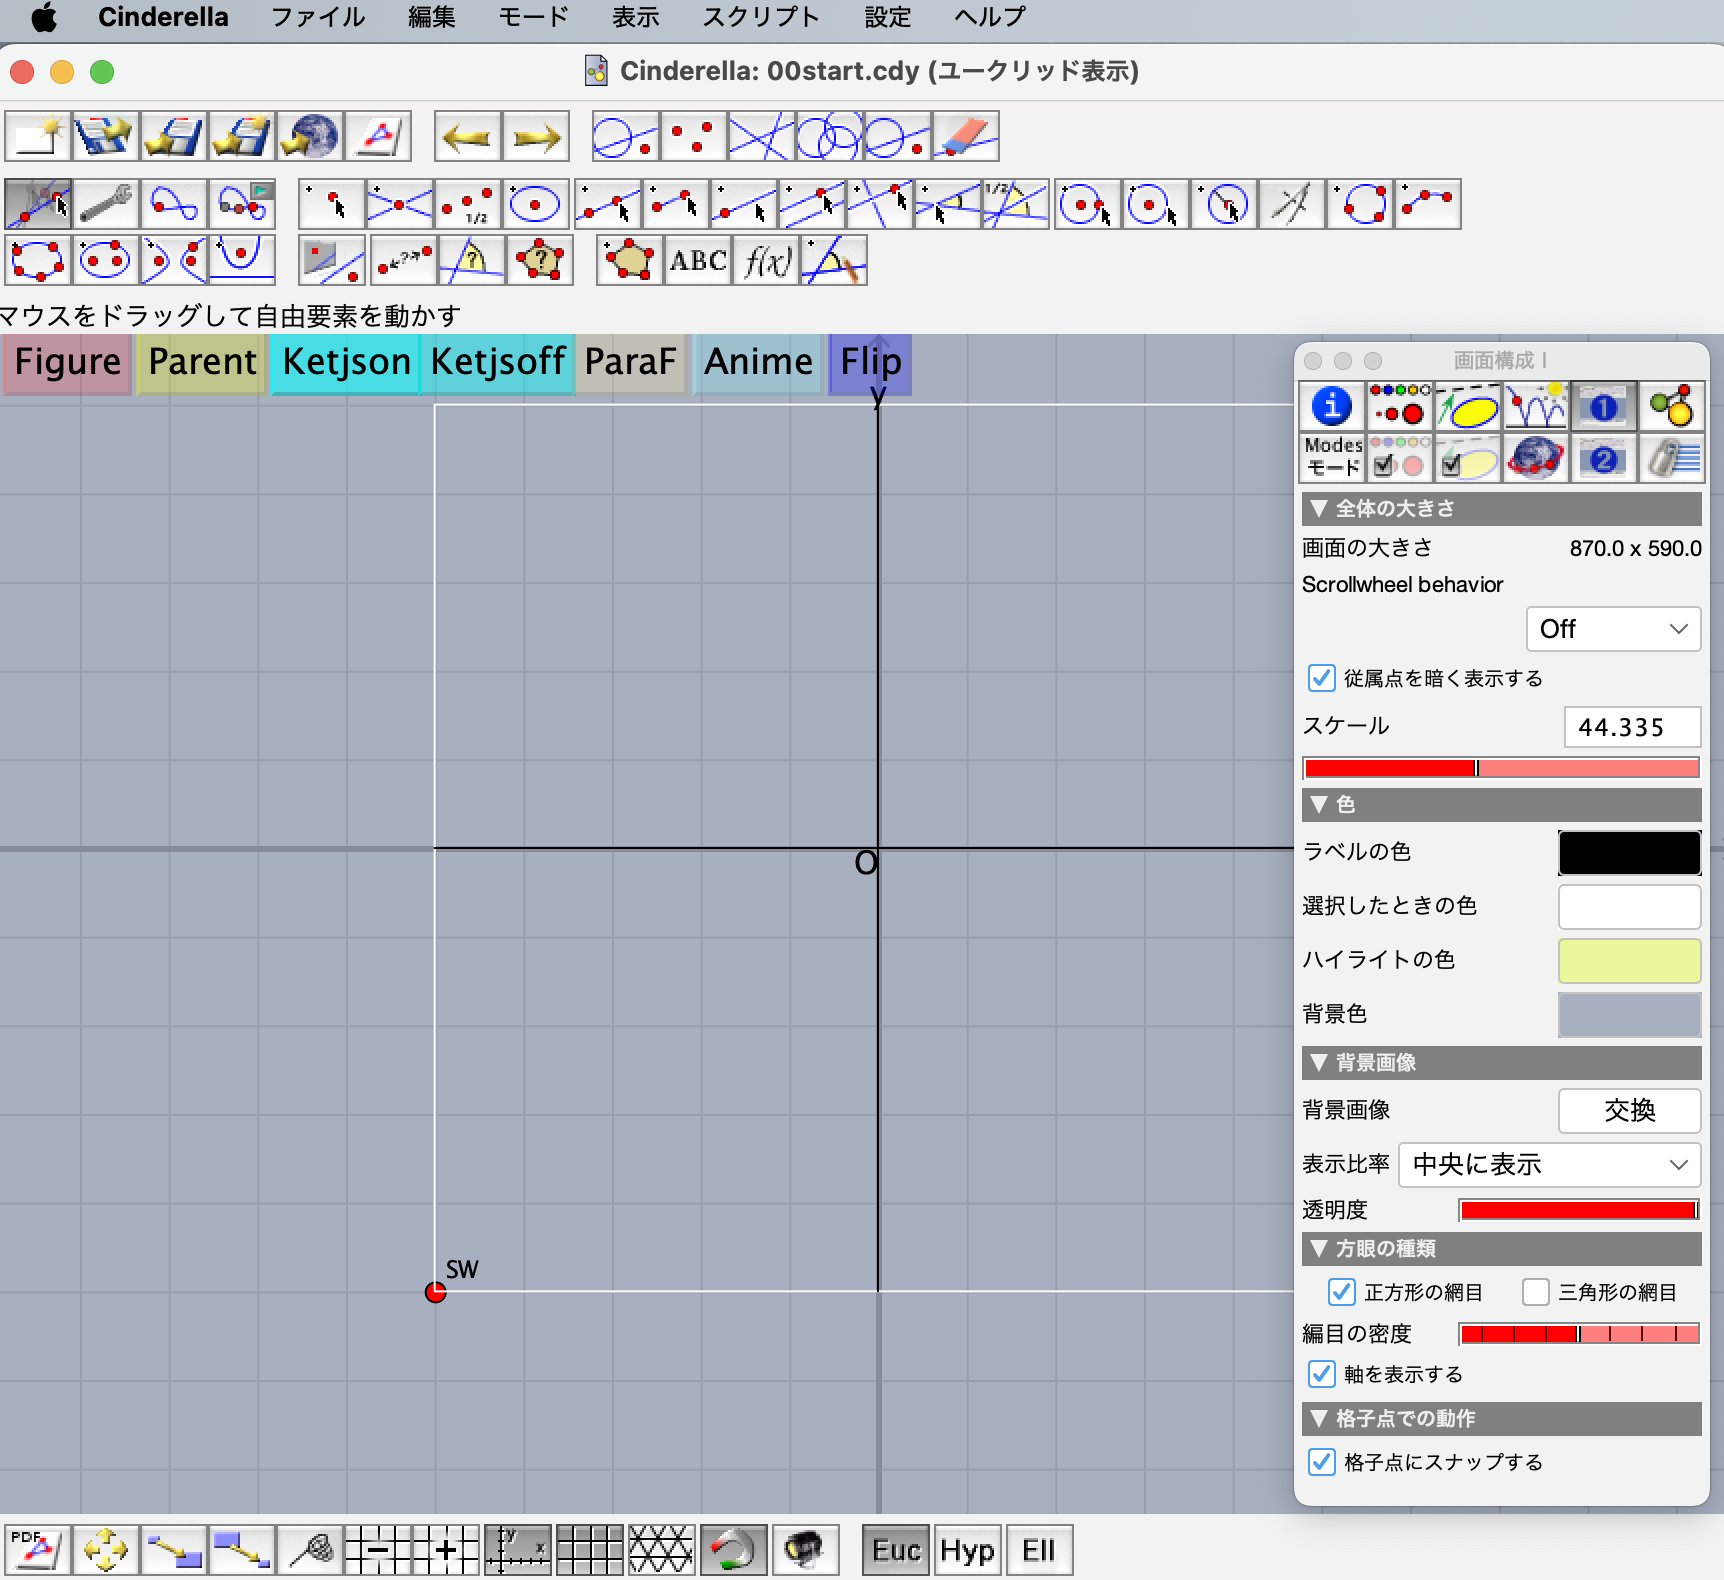
\includegraphics[bb=0 0 1724 1584,width=38mm]{2.png}}
\putnotesw{120}{40}{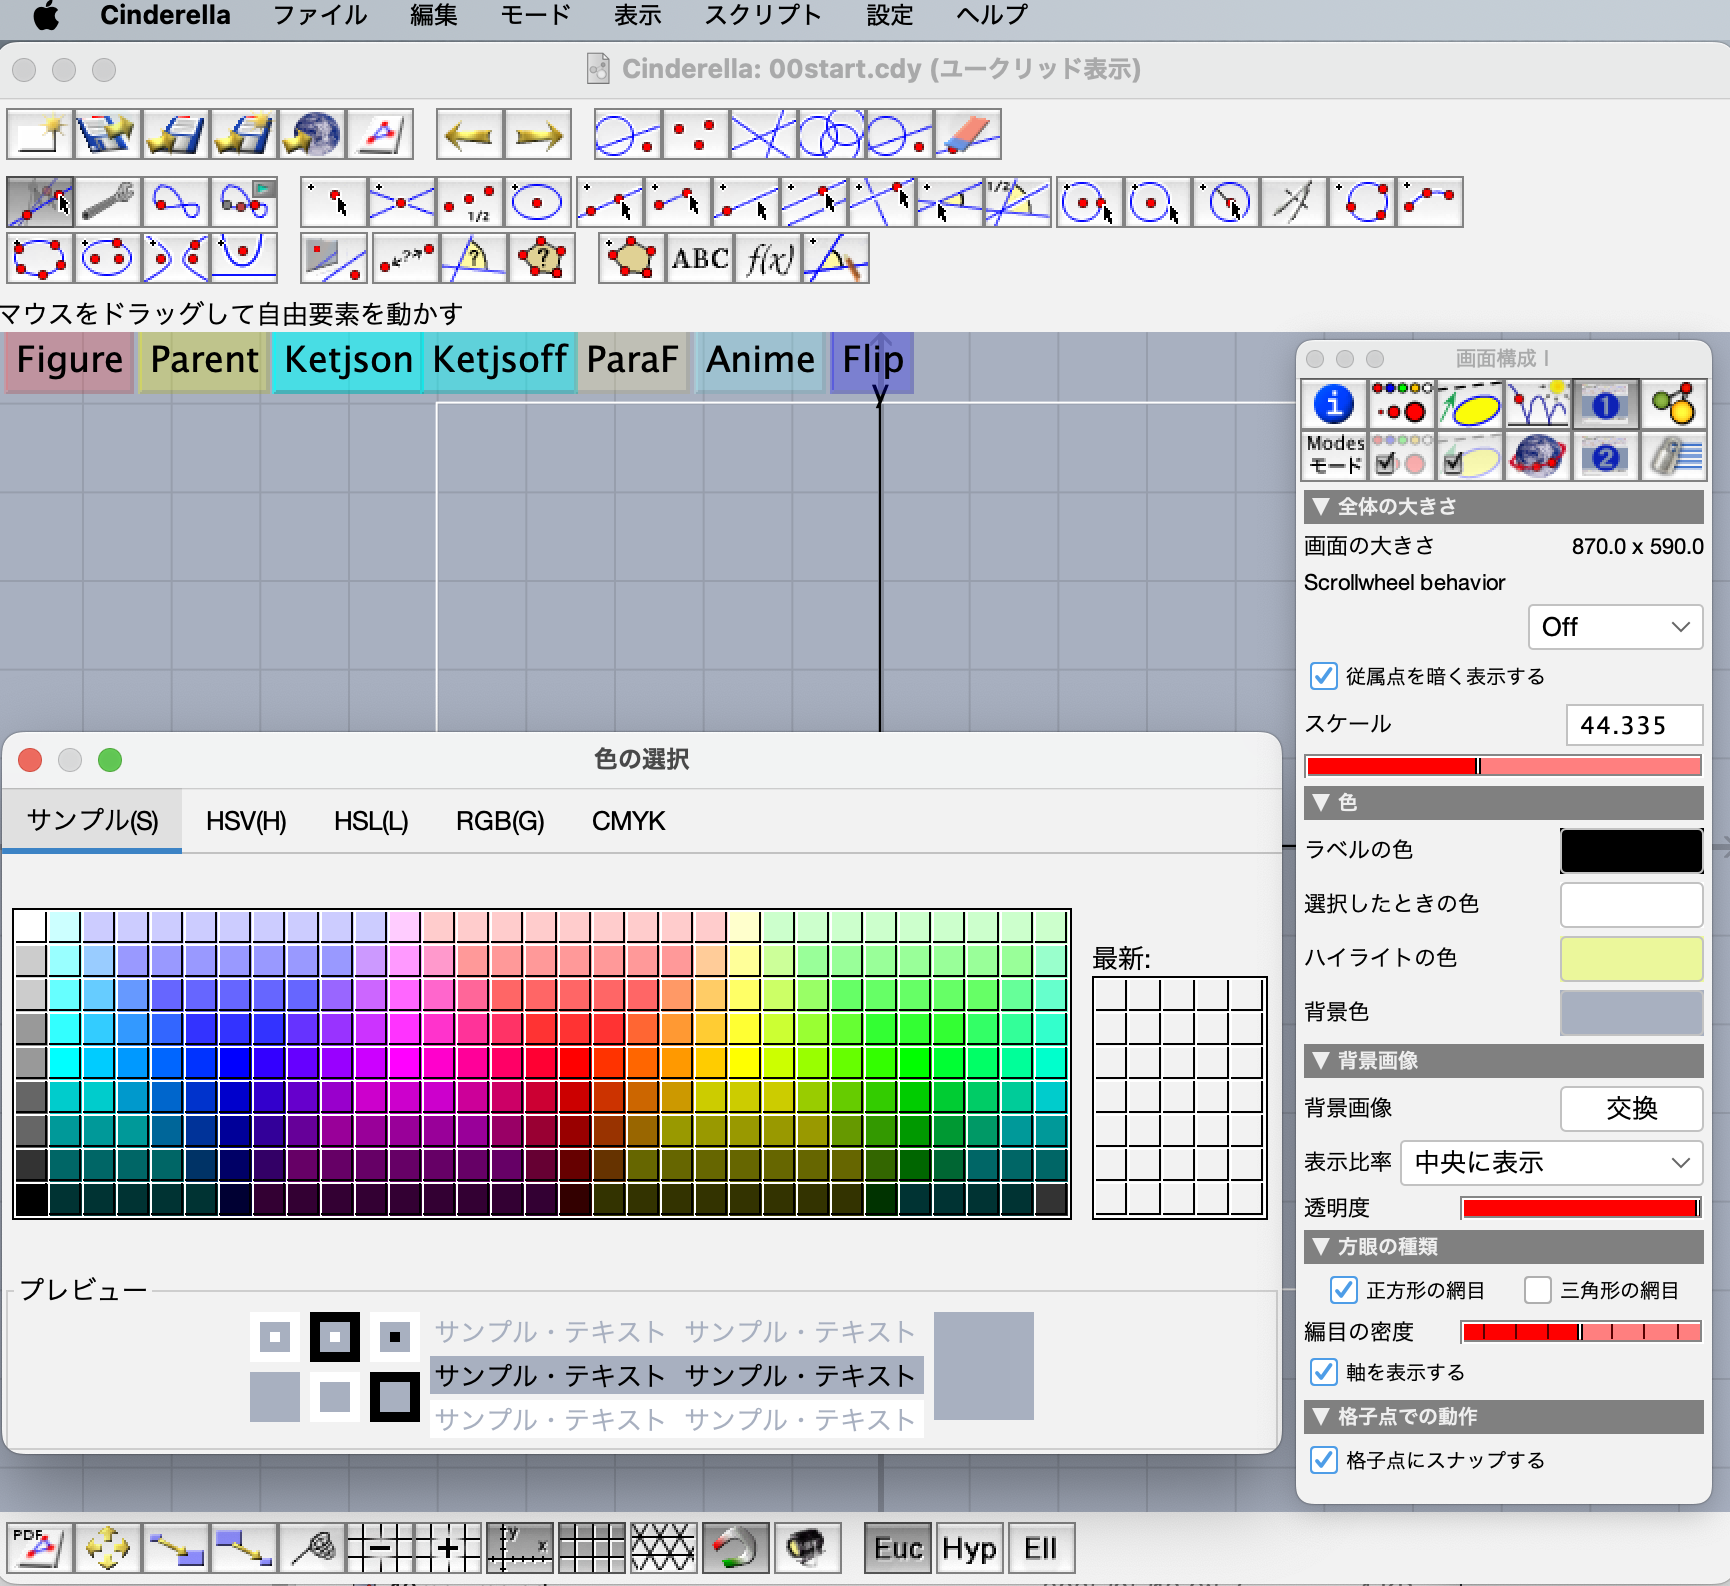
\includegraphics[bb=0 0 1724 1584,width=38mm]{3.png}}
\putnotesw{170}{40}{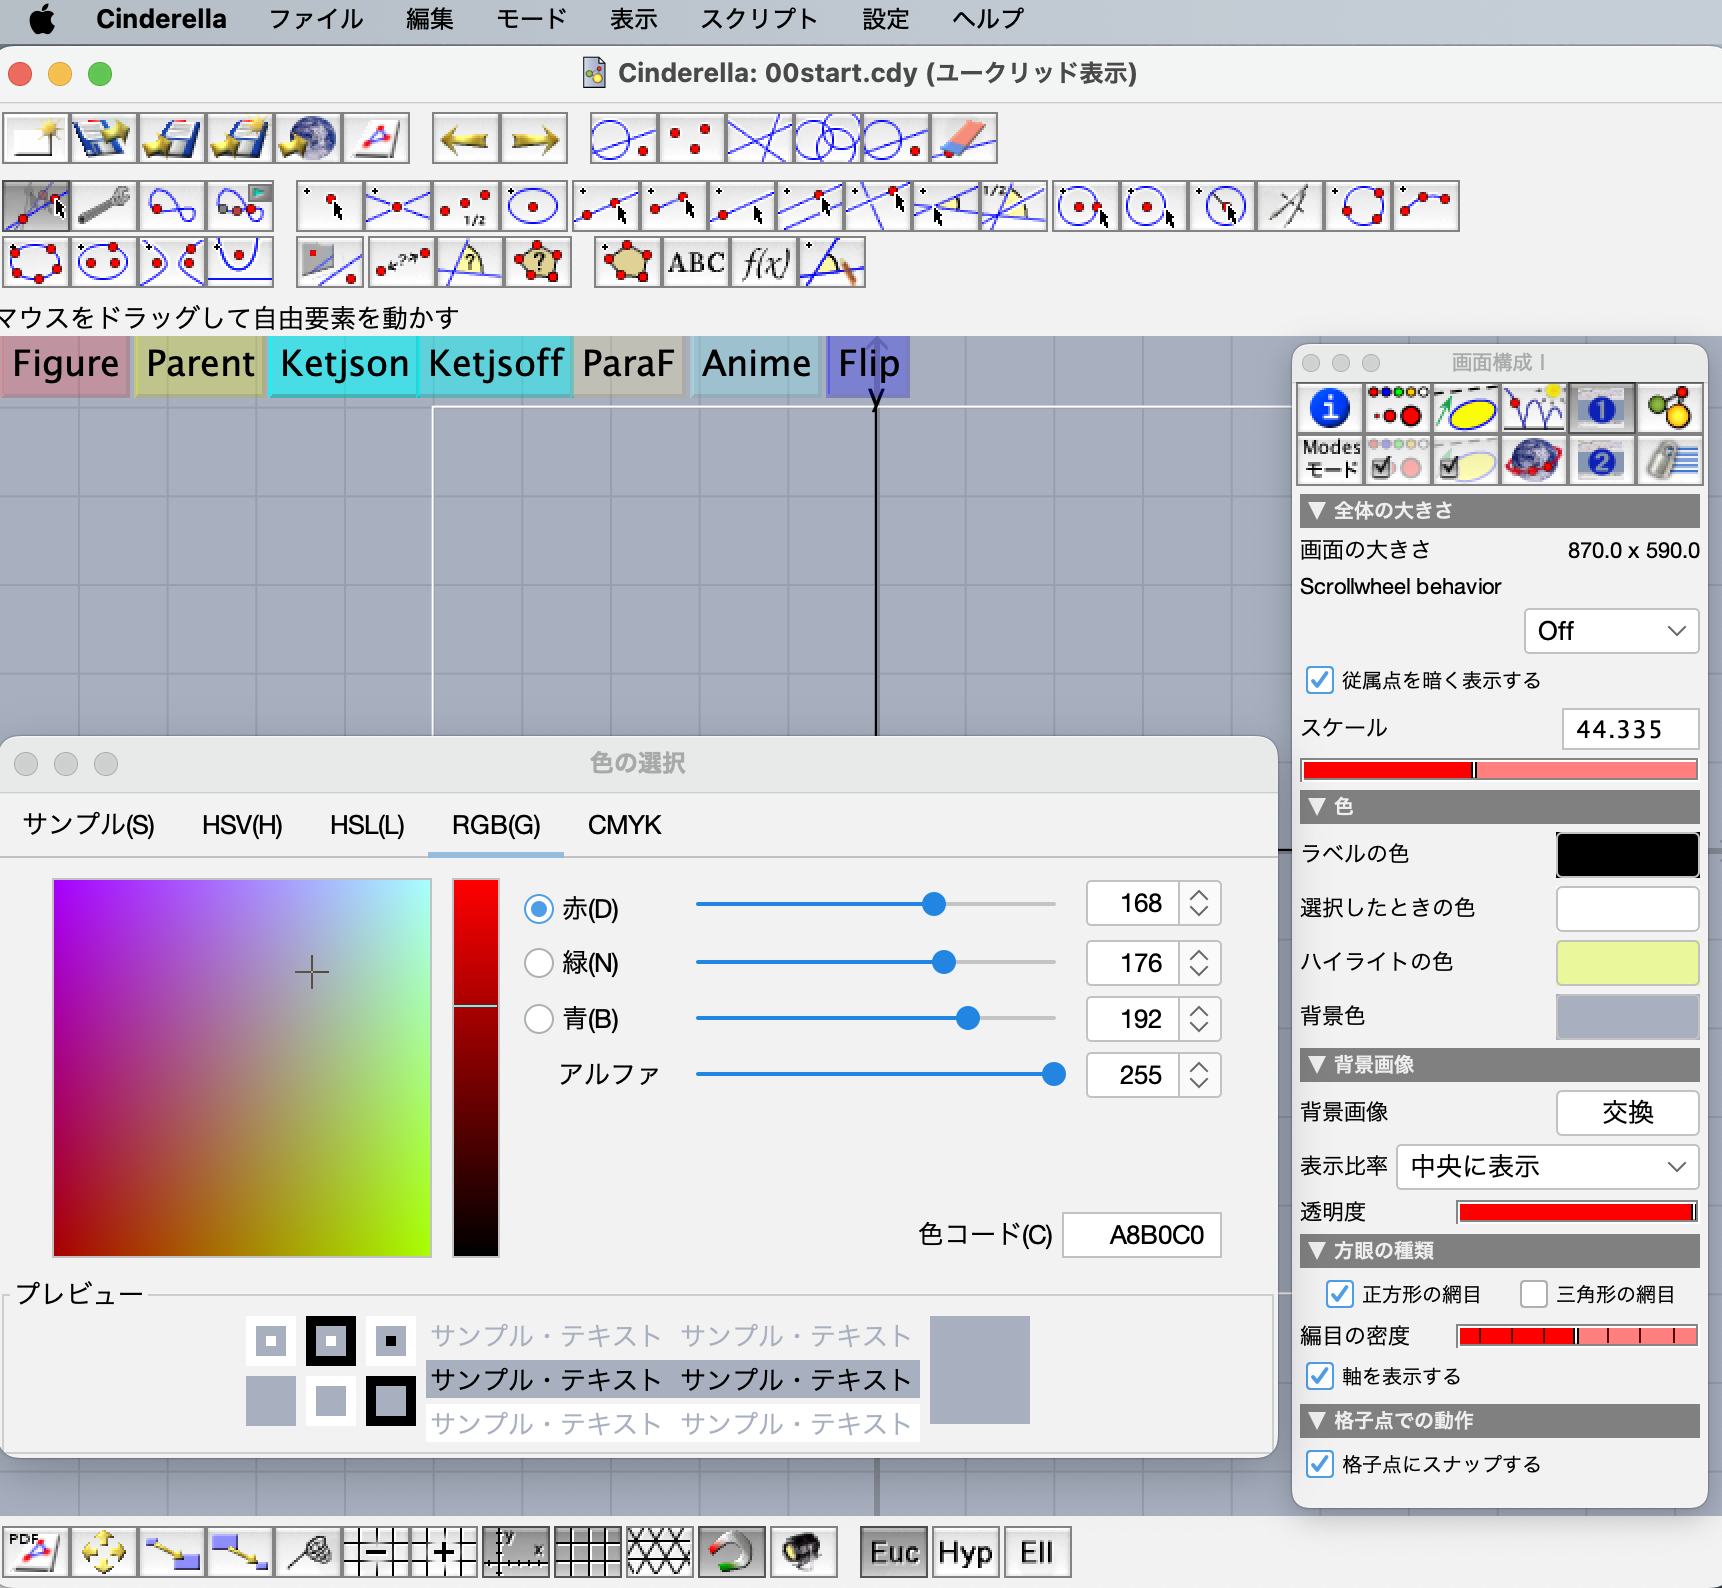
\includegraphics[bb=0 0 1724 1584,width=38mm]{4.png}}
\end{layer}


\begin{minipage}{.38\textwidth}{「情報を見る」のショートカット,または,メニューから
[編集]→[インスペクタ]で,図1の右端のようなメニューを出したら,上の段の右から2番目をクリックし,\\
図2の右端の窓のように縦に長い窓にして,
その中の背景色をクリックして,\\
図3のような中央のように色を選べるようにします。\\
参考:RGBタブをクリックして図4のようにすれば,初期値に戻せます。
初期値は,\\
RGBなら\\
R:168,
G:176,
B:192,
アルファ:255
です。}
\end{minipage}
\end{document}
